%%%%%%%%%%%%%%%%%%%%%%%%%%%%%%%%%%%%%%%%%%%%%%%%%%%%%%%%%%%%%%%%%%%%%%%%%%%%%%%%%%%%%%%%%%%%%%%%%%%%%%%%%%%%%%%%%%%%%%%%
%																													   %
%								     				LaTeX-Kurs 2020													   %
%																													   %
%%%%%%%%%%%%%%%%%%%%%%%%%%%%%%%%%%%%%%%%%%%%%%%%%%%%%%%%%%%%%%%%%%%%%%%%%%%%%%%%%%%%%%%%%%%%%%%%%%%%%%%%%%%%%%%%%%%%%%%%

% TODO häufigste Fehler listen
% TODO Gotchas
%   * Leerzeichen nach Befehl --> \befehl\
%   * nicht erlaubt ohne $$ (Missing $ inserted. Hallo Welt t_)
%   * fehlende Einheit
% TODO Beamer
% TODO listings

\documentclass[titlepage, parskip=full*]{scrartcl}

\usepackage[utf8]{inputenc}
\usepackage[T1]{fontenc}

% Ladereihenfolge der Fonts ist wichtig!
%   1) libertine für Titel und Überschriften setzen mit \addtocomafont
%   2) libertine mit lmodern überschreiben als Font für den Text
%   3) lmodern mit eulervm überschreiben als Font für Mathe-Modus
\usepackage{libertine}
\usepackage{lmodern}
\addtokomafont{title}{\libertine\color{white}}
\addtokomafont{author}{\libertine}
\addtokomafont{date}{\libertine}
\addtokomafont{section}{\libertine}
\addtokomafont{subsection}{\libertine}
\addtokomafont{subsubsection}{\libertine}
\usepackage{eulervm}

% microtype verfeinert den Textsatz durch flexible Zwischenräume etc.
\usepackage{microtype}
\usepackage[bottom=3cm]{geometry}
\usepackage[ngerman]{babel}
\usepackage[style=german]{csquotes}
\usepackage{amsmath, amssymb, amsfonts}
\usepackage{graphicx, caption}
\usepackage{hyperref}

\usepackage{listings}
\usepackage{xcolor}
\definecolor{lsnumber}{rgb}{0,0,0} % Zeilennummerfarbe
\definecolor{lscomment}{rgb}{0.25,0.5,0.35} % Kommentarfarbe
\definecolor{lskeyword}{rgb}{0.5,0,0.35} % Schlüsselwörterfarbe
\definecolor{lsstring}{rgb}{0.6,0,0} % Zeichenkettenfarbe
\lstset{language=[LaTeX]{TeX},
    tabsize=4,
    keepspaces=true,
    breakatwhitespace=true,
    breaklines=true,
    prebreak={\mbox{$\hookleftarrow$}},
    basicstyle=\ttfamily,
    numbers=left,
    stepnumber=1,
    numbersep=8pt,
    numberstyle=\color{lsnumber}\small,
    commentstyle=\color{lscomment},
    keywordstyle=\bfseries\color{lskeyword},
    stringstyle=\color{lsstring},
    extendedchars=true,
    inputencoding=utf8,
    literate={ä}{{\"a}}1 {ö}{{\"o}}1 {ü}{{\"u}}1 {ß}{{\ss}}1,
    morekeywords={tableofcontents, includegraphics, subsection, text, succcurlyeq, intertext}
}
\renewcommand{\lstlistingname}{Code}

\usepackage{totpages}
\usepackage[headsepline,footsepline]{scrlayer-scrpage}
\pagestyle{scrheadings} 
\clearscrheadfoot
\ihead{\LaTeX-Einführung des FSR Mathe/Info an der MLU Halle-Wittenberg}
\cfoot[\thepage/\ref{TotPages}]{\thepage/\ref{TotPages}} 
\setkomafont{pageheadfoot}{\sffamily\libertine} 
\setkomafont{pagination}{\sffamily}

% Setze parskip in minipage auf gleichen Wert wie im Dokument.
\newlength{\currentparskip}
\setlength{\currentparskip}{\parskip}

\widowpenalties=4 10000 10000 150 0

\definecolor{mlugreendark}{rgb}{0.11, 0.29, 0.2}
\definecolor{mlugreenlight}{cmyk}{0.45,0,0.90,0}
\definecolor{mlugreenlightarea}{rgb}{0.52, 0.81, 0.29}

\author{Luis Imsande\and Fachschaftsrat Mathematik/Informatik\\Martin-Luther-Universität Halle-Wittenberg}
\title{\Huge Einführung in \LaTeX}
\date{}


\begin{document}
\pagecolor{mlugreenlightarea}
\maketitle



\pagecolor{white}
\thispagestyle{empty}
\vspace*{\stretch{1}}
\minisec{Impressum}
\begin{tabbing}
\hspace{3cm}\=\kill
Herausgeber \> Fachschaftsrat Mathematik/Informatik der Studierendenschaft \\
\> der Martin-Luther-Universität Halle-Wittenberg K.d.ö.R. \\ 
Autor \> Luis Imsande \\
Kontakt \> limsande@yahoo.com
\end{tabbing} 

Gesetzt mit \LaTeX
\newpage



\setcounter{page}{1}
\tableofcontents
\newpage



%-----------------------------------------------------------------------------------------------------------------------

\section{Über dieses Dokument}
Dieses Dokument, inklusive sein \LaTeX-Quellcode, ist frei verfügbar auf GitHub.com\footnote{\url{https://github.com/Limsande/latex-intro.git}}. Es ist gedacht als ausführliche Form des Crashkurses zum Textsatzsystem \LaTeX\ der Fachschaft Mathematik/Informatik an der Martin-Luther-Universität Halle-Wittenberg. Es ist definitiv keine vollständige Beschreibung von \LaTeX\ und all seinen Funktionen, sondern soll nur das vermitteln, was wir für den Einstieg wichtig finden. Nach dem Lesen sollten zusammen mit den Inhalten des Kurses das Erstellen von Lösungen der Übungsserien der ersten Semester gut möglich sein.

Um den Einstieg noch einfacher zu machen, hat der FSR eine Vorlage für die Übungsserien erstellt, die praktisch alle Einstellungen automatisch vornimmt. Es muss also nur noch der Text eingefügt werden. Diese Vorlage wurde im Kurs vorgestellt und steht auf unserer Website\footnote{\url{https://fachschaft.mathinf.uni-halle.de}} zur Verfügung. Einiges, was hier erklärt wird, nimmt euch die Vorlage bereits ab.

Im Kurs wurde als Arbeitsumgebung der Online-\LaTeX-Editor Overleaf\footnote{\url{www.overleaf.com}} vorgestellt. Eine Online-Lösung halten wir für besonders einfach, da so die ganze Administration einer eigenen \LaTeX-Installation entfällt und nichts auf dem eigenen Rechner installiert werden muss. Deshalb wird hier auch keine Installationshilfe gegeben, lediglich die bekanntesten Distributionen erwähnt. Trotzdem stehen wir natürlich immer für Fragen, nicht nur zum Thema \LaTeX, zur Verfügung, z. B. über unsere Webseite\footnote{\url{https://fachschaft.mathinf.uni-halle.de/kontakt/}}. Außerdem bietet das Institut für Informatik den Informatik-Treff\footnote{\url{https://www.informatik.uni-halle.de/studium/informatik-treff/}} an, wo euch Studenten höherer Semester bei Fragen zur Seite stehen. In Abschnitt \ref{sec:hilfe} am Ende des Dokuments ist eine Sammlung von Links zu \LaTeX-Hilfen.



%-----------------------------------------------------------------------------------------------------------------------

\section{Was ist \LaTeX?}\label{sec:was_ist_das}
\LaTeX\ (sprich: Latech) ist ein Textsatzsystem. Seine Stärken liegen ganz besonders bei mathematischen und technischen Darstellungen. \LaTeX\ ist tatsächlich eine Erweiterung des Textsatzsystems \TeX\ aus dem Jahr 1978, welches entwickelt wurde aus dem damaligen Mangel an Möglichkeiten, mathematische und generell wissenschaftliche Texte in hoher Qualität zu setzen. Heute ist \LaTeX\ de-facto Standard für wissenschaftliche Arbeiten. Es ist \emph{open source}, d. h. sein Programmcode ist für jeden frei einsehbar, und für alle gängigen Betriebssysteme verfügbar. Dieses Dokument wurde übrigens auch mit \LaTeX\ erstellt.


\subsection{WYSIWYG vs. WYSIWYM}
Systeme zum Erstellen von Texten lassen sich in die Kategorien \enquote{WYSIWYG} (\emph{\enquote{What you see is what you get}}) und \enquote{WYSIWYM} (\emph{\enquote{What you see is what you mean}}) einteilen. Zur ersten Kategorie gehören z. B. Office-Programme wie Microsoft Word und LibreOffice. Im Grunde bedeutet \enquote{WYSIWYG}: Was ich in meinem Editor während des Schreibens sehe, ist bereits das fertige Dokument (Schreiben des Textes und Erstellen des Dokumentes ist also ein einziger Schritt). 

\LaTeX\ gehört zur zweiten Kategorie, bei der der Prozess aus zwei Schritten besteht: Der im Editor erstellte Text ist nur eine Rohfassung (\enquote{Quelldatei}). Damit daraus ein fertiges Dokument wie bspw. ein PDF wird, muss er durch ein Programm verarbeitet (\enquote{übersetzt} oder \enquote{kompiliert}) werden. Erst dabei wird der Text mit vorher festgelegten Einstellungen formatiert (Schriftgröße, Schriftart, Hervorheben von Überschriften etc.), Abbildungen werden an vorher definierten Stellen eingefügt, Verweise generiert u.v.m.

Da die Formatierung komplett von \LaTeX\ übernommen wird, kann es viele Dinge für das fertige Dokument optimieren. \LaTeX\ ist z. B. bestrebt, alle Absätze, Abbildungen, Tabellen etc. so auf die einzelnen Seiten des Dokuments aufzuteilen, das jede einzelne Seite so gut aussieht wie möglich.



\subsection{Zur Arbeit mit \LaTeX}
Der Quellcode ist im Grunde eine Textdatei (\texttt{.txt}) mit der Endung \texttt{.tex} und kann daher prinzipiell mit jedem Texteditor erstellt werden. Spezielle \LaTeX-Editoren wie Texmaker\footnote{\url{https://www.xm1math.net/texmaker/}} erleichtern einem das Leben allerdings mit einigen Features wie intelligenter Vervollständigung und automatischem Syntaxcheck. Webbasierte Editoren wie Overleaf\footnote{\url{https://www.overleaf.com/}} bieten außerdem die Möglichkeit, Dokumente gemeinsam in Echtzeit zu bearbeiten.

Möchte man \LaTeX\ lieber lokal auf dem eigenen Rechner benutzen (was wir für den Einstieg nicht empfehlen), muss etwas Software installiert werden. Zwei gängige Distributionen des gesamten \LaTeX-Systems, das zur Übersetzung gebraucht wird, sind TeX Live \footnote{\url{http://tug.org/texlive/}} und MiKTeX\footnote{\url{https://miktex.org/}}.

\subsubsection{Befehle}
Das Programm, das aus \LaTeX-Quellcode ein PDF erstellt, heißt \texttt{pdflatex}. Beim Übersetzen durchsucht es die Quelldatei nach speziellen Wörtern (\enquote{Befehlen}), die ihm sagen, wie es den Text verarbeiten soll. Ein \LaTeX-Befehl beginnt mit einem Backslash (\textbackslash). Beispiele sind \lstinline|\tableofcontents|, \lstinline|\textbf{}| und \lstinline|\begin{equation}|. An diesen Beispielen sind drei verschiedene Typen von \LaTeX-Befehlen zu sehen:

\begin{itemize}
\item Einfache, parameterlose Befehle stehen für sich und können verschiedenste Auswirkungen haben. \lstinline|\tableofcontents| z. B. erzeugt ein Inhaltsverzeichnis des Dokuments.

\item Befehle mit Parameter(n) benötigen zusätzliche Angaben, um zu funktionieren. Diese werden in geschweiften Klammern (\verb|{}|) übergeben: \lstinline|\textbf{Hallo}| führt dazu, dass \enquote{Hallo} (der Parameter) fett gedruckt wird, \lstinline|\section{Thema X}| erzeugt eine Überschrift mit dem Namen \enquote{Thema X}.

Befehle können außerdem \emph{optionale} Parameter haben, d. h. zusätzliche Parameter, die nicht unbedingt angegeben werden müssen, der Befehl funktioniert auch ohne sie. Diese werden in eckigen Klammern ([ ]) geschrieben. Ein Beispiel ist \lstinline|\includegraphics[width=10cm]{bild.png}|, wodurch das Bild \enquote{bild.png} in das Dokument eingefügt und zusätzlich auf eine Breite von 10\,cm skaliert wird. Ohne \texttt{[width=10cm]} würde das Bild in der Originalgröße eingefügt.

\item Befehle zum Öffnen und Schließen von Umgebungen: \lstinline|\begin{}| und\lstinline|\end{}|. Eine Umgebung ist ein Bereich, in dem bestimmte Regeln für die Formatierung gelten. Die \texttt{equation}-Umgebung z. B. stellt ihren Inhalt als einzeilige mathematische Gleichung da, zentriert mit etwas Abstand darüber und darunter (wie man sie benutzt, wird in Abschnitt \ref{sec:math} erklärt). Einige Befehle sind nur in einer bestimmten Umgebung erlaubt.
\end{itemize}

Ganz allgemein markieren Befehle also Textstellen und bestimmen so, wie diese später im fertigen Dokument aussehen werden. Diese Form des Textsatzes nennt man auch \emph{logisches Markup}.

Stößt \texttt{pdflatex} beim Übersetzen auf einen unbekannten Befehl (z. B. wegen eines Tippfehlers) oder eine andere Unstimmigkeit (beliebt sind fehlende schließende Klammern), bricht es mit einer Fehlermeldung ab und erzeugt kein PDF. In der Meldung steht meistens die Zeilennummer, in der der Fehler entdeckt wurde, diese ist jedoch nicht immer korrekt, da die eigentliche Ursache bereits früher aufgetreten sein kann.

\subsubsection{Kommentare}
Eine besondere Bedeutung hat das Prozentzeichen (\%). Immer wenn \texttt{pdflatex} diesem Zeichen begegnet, ignoriert es alles weitere bis zum Ende der aktuellen Zeile. Text, der nach einem \% steht, ist für das Programm also praktisch unsichtbar. Das ist eine einfache Möglichkeit, sich selbst Notizen in den Quellcode zu schreiben, wie \lstinline|% Todo| oder \lstinline|% geklaut von stackoverflow.com|. Zur Benutzung von Kommentaren siehe Abschnitt \ref{sec:formatierung_und_struktur}.



%-----------------------------------------------------------------------------------------------------------------------

\section{Ein minimales \LaTeX-Dokument}\label{sec:hallo_welt}
Jedes \LaTeX-Dokument muss mindestens die folgenden Dinge beinhalten:

\begin{minipage}{.49\linewidth}
	\lstinputlisting[caption=Minimales \LaTeX-Dokument]{input/hallo_welt.tex}
\end{minipage}
\fbox{
\begin{minipage}{.49\linewidth}
    Hallo Welt!
\end{minipage}
}

Der Text in den Zeilen 3 und 4 ist natürlich austauschbar. An dieser Stelle wird der tatsächliche Inhalt des Dokuments eingefügt. Wie bereits erwähnt, erscheinen Kommentare nicht im fertigen PDF. Zeilenumbrüche, die mit $\hookleftarrow$ gekennzeichnet sind, existieren nicht im Quellcode. Sie kommen nur wegen des begrenzten Platzes für die Darstellung zustande.

\begin{description}
\item[Zeile 1] Der Befehl \lstinline|\documentclass{}| muss immer der erste \LaTeX-Befehl eines Dokuments sein. Er definiert, um was für eine Art von Dokument es sich handeln soll. Die Klasse \texttt{article} z. B. steht für einen kurzen Text, wie eine wissenschaftliche Publikation in einer Fachzeitschrift (\emph{Paper}). Für längere Aufsätze, wie Fach- und Abschlussarbeiten, eignet sich \texttt{report}. Die Wahl der Klasse hat vor allem Auswirkungen darauf, wie \LaTeX\ das Dokument formatiert (siehe auch Kapitel \ref{sec:klassen}). Für Übungsserien an der MLU eignet sich die Vorlage des FSR besonders gut.

\item[Zeile 2] Der Befehl \lstinline|\begin{document}| markiert den Anfang des eigentlichen Dokuments. Alles ab hier wird später im PDF zu sehen sein.

\item[Zeile 3] Zwischen \lstinline|\begin{document}| und \lstinline|\end{document}| kann Text geschrieben, Bilder eingefügt werden u.v.m. (die sogenannte \texttt{document}-Umgebung).

\item[Zeile 4] Der Befehl \lstinline|\end{document}| signalisiert \LaTeX, dass das Dokument zu Ende ist. Alles danach wird ignoriert.
\end{description}

Durch das Übersetzen dieses Codes erhält man eine einzelne Seite mit dem Satz \enquote{Hallo Welt!} wie rechts neben dem \LaTeX-Code dargestellt.



%-----------------------------------------------------------------------------------------------------------------------

\section{Schriftformatierung \& Dokumentstruktur}\label{sec:formatierung_und_struktur}


\subsection{Absätze und Umbrüche}
Zwei Absätze werden durch eine komplett leere Zeile im Quellcode gekennzeichnet. Zeilenumbrüche müssen i. d. R. nicht von Hand eingefügt werden, da \LaTeX\ automatische Silbentrennung beherrscht. Will man eine Zeile trotzdem an einer bestimmten Stelle umbrechen, geht dies mit \lstinline|\\|. Ein \enquote{einfacher} Zeilenumbruch durch drücken der Entertaste funktioniert nicht, da \LaTeX\ diesen nur als ein Leerzeichen ansieht. Ein Seitenumbruch lässt sich mit \lstinline|\pagebreak| oder \lstinline|\newpage| erzeugen.

\begin{minipage}{.49\linewidth}
	\lstinputlisting[caption=Umbrüche und Kommentare]{input/absatz.tex}
\end{minipage}
\fbox{
\begin{minipage}{.49\linewidth}
	\setlength{\parskip}{\currentparskip}
	Ein Absatz.

Noch ein Absatz. Und ein\\
Zeilenumbruch. Und kein
Zeilenumbruch.
\end{minipage}
}


\subsection{Schriftgröße etc.}
Die Schriftgröße (voreingestellt ist meistens 12) lässt sich u. a. mit den Befehlen \lstinline|\tiny| und \lstinline|\huge| verändern. Zurücksetzen auf die normale Größe geht mit \lstinline|\normalsize|. Die Auswirkung lässt sich auch durch geschweifte Klammern (\verb|{}|) begrenzen.

\begin{minipage}{.49\linewidth}
	\lstinputlisting[caption=Schriftgröße]{input/schriftgroesse.tex}
\end{minipage}
\fbox{
\begin{minipage}{.49\linewidth}
	\setlength{\parskip}{\currentparskip}
	Dieser Text ist normal groß. 
Jetzt wird's \tiny winzig. 
Groß wird es \huge jetzt. 
Zurück zu normal: \normalsize 
ab hier. Einzelnes {\tiny Wort}
geht so.
\end{minipage}
}

Der Schrifttyp, also fett, kursiv etc., lässt sich über folgende Befehle einstellen; dabei steht \enquote{bf} für \emph{boldface}, \enquote{it} für \emph{italics} und \enquote{tt} für \emph{teletype} (die englischen Begriffe für fett, kursiv und Schreibmaschinenschrift):

\begin{minipage}{.49\linewidth}
	\lstinputlisting[caption=Schrifttyp]{input/schrifttyp.tex}
\end{minipage}
\fbox{
\begin{minipage}{.49\linewidth}
	\setlength{\parskip}{\currentparskip}
	Dieses Wort ist \textbf{fett}, 
\textit{kursiv}, 
\textbf{\textit{fett-kursiv}}, 
\texttt{monospace}.
\end{minipage}
}


\subsection{Titel \& Dokumentkopf}
Das Dokument lässt sich mit einem Kopf versehen bestehend aus Titel, Autor und Datum mit Hilfe des Befehls \lstinline|\maketitle|. Um zu funktionieren, müssen dafür natürlich Titel, Autor und Datum angegeben werden. Das geht mit den Befehlen \lstinline|\title{Beispieltitel}|, \lstinline|\author{Beispielautor}| und \lstinline|\date{Beispieldatum}|. Diese müssen \emph{vor} \lstinline|\maketitle| stehen. Der Kopf wird genau da eingefügt, wo \lstinline|\maketitle| im Quellcode steht (in aller Regel direkt nach \lstinline|\begin{document}|). Das Hallo-Welt-Beispiel sieht mit Dokumentkopf so aus:

\begin{minipage}{.49\linewidth}
	\lstinputlisting[caption=Dokumentkopf]{input/hallo_welt_mit_titel.tex}
\end{minipage}
\fbox{
\begin{minipage}{.49\linewidth}
	\setlength{\parskip}{\currentparskip}
	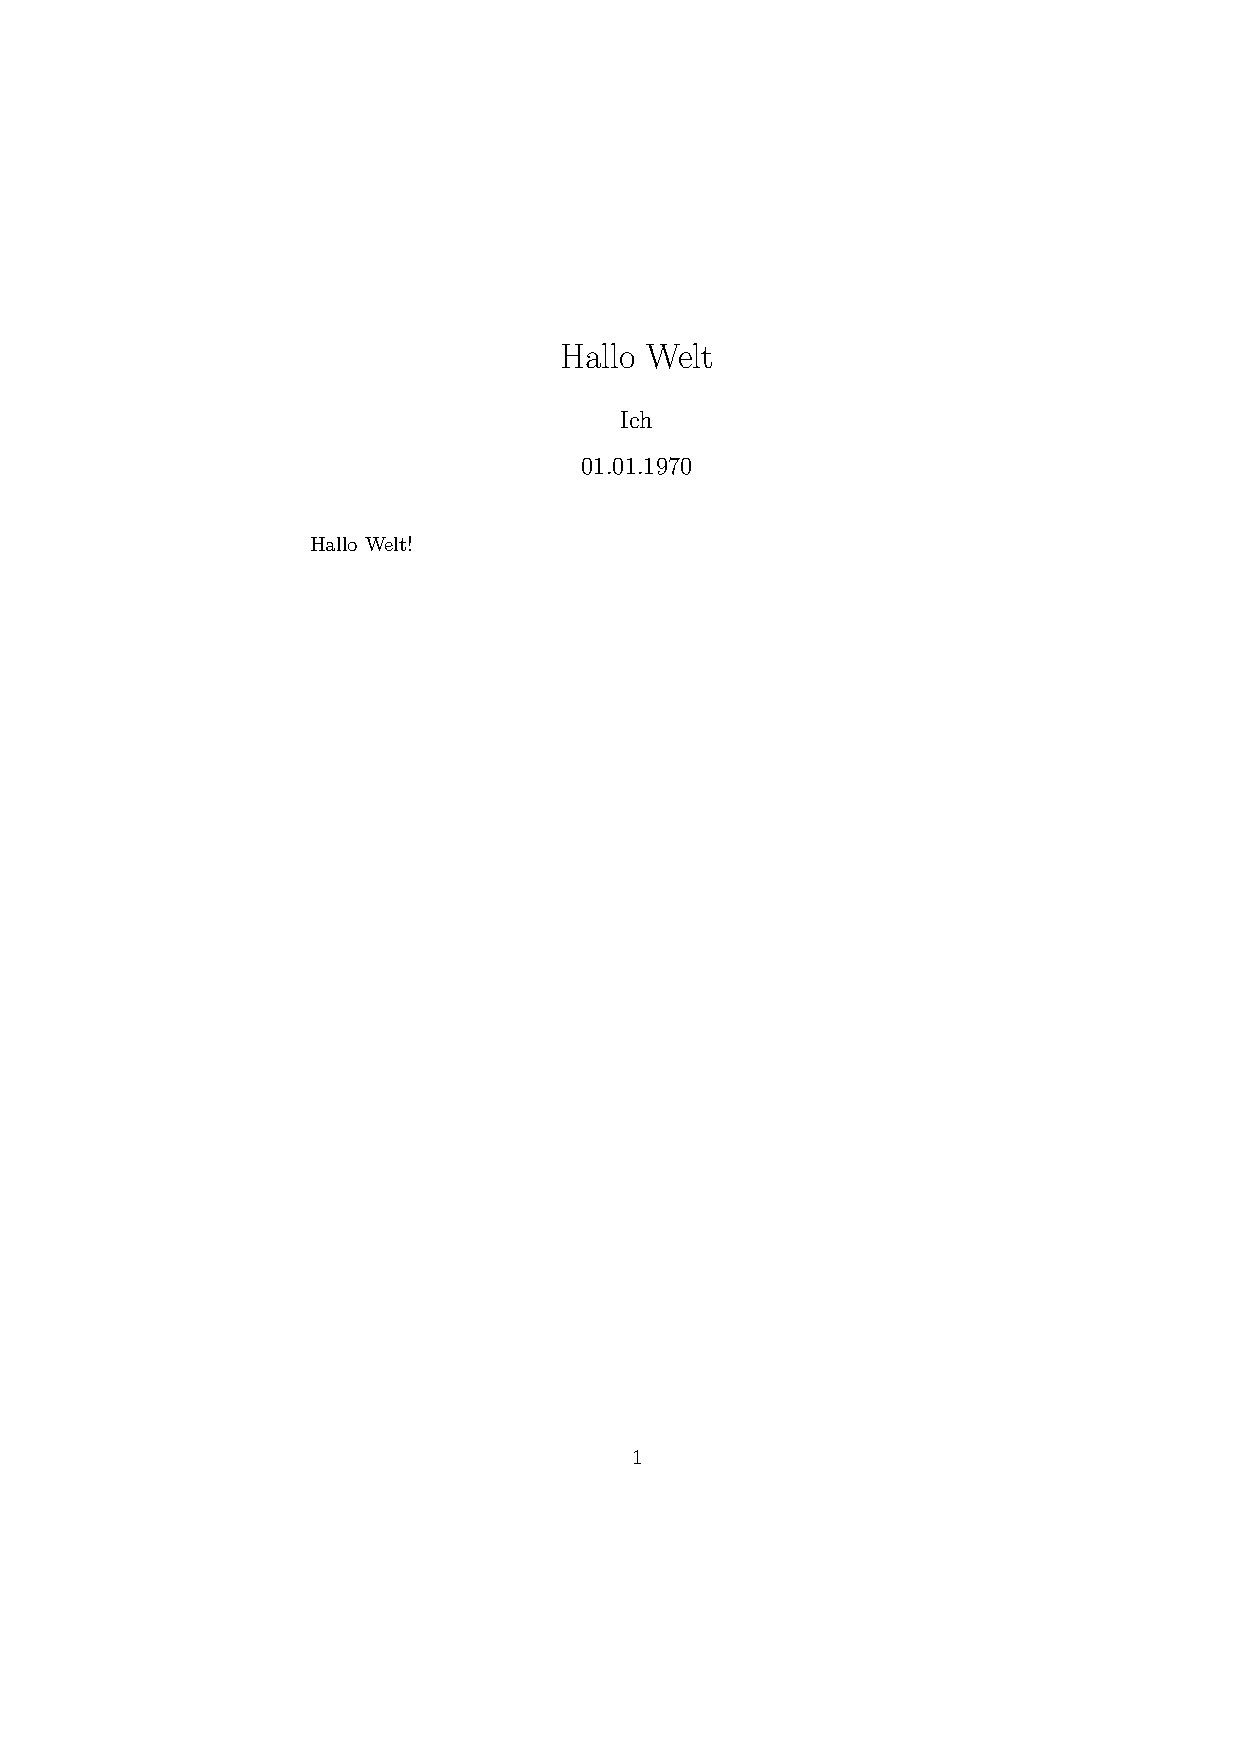
\includegraphics[width=\linewidth]{input/hallo_welt_mit_titel.pdf}
\end{minipage}
}

Soll kein Datum ausgegeben werden, kann \lstinline|\date{}| auch leer gelassen werden. Wird \lstinline|\date{}| ganz weggelassen, wird automatisch das aktuelle Datum eingefügt.


\subsection{Gliederung (Zwischenüberschriften)}
Die Gliederung des Dokuments (also einzelne Abschnitte mit Überschriften) kann mit den Befehlen \lstinline|\section{Name}| und \lstinline|\subsection{Name}| vorgenommen werden. Tiefere Gliederungsebenen gibt es auch, die benötigt man aber fast nie und werden deshalb nicht weiter erwähnt. Überschriften werden automatisch in Schriftgröße und -typ vom Text abgehoben und mit einer fortlaufenden Nummer versehen. Letzteres lässt sich durch die Varianten \lstinline|\section*{Name}| und \lstinline|\subsection*{Name}| unterdrücken. Mit dem Befehl \lstinline|\tableofcontents| kann ein Inhaltsverzeichnis inklusive Seitenangaben erstellt werden.



%-----------------------------------------------------------------------------------------------------------------------

\section{Funktion erweitern mit Paketen}\label{sec:pakete}
Obwohl in \LaTeX\ standardmäßig schon viel Funktionalität enthalten ist, reicht diese nicht immer aus. Für das Einfügen von Bildern oder komplexen Formelsatz (um nur zwei Beispiele zu nennen) muss sie erweitert werden. Das geht durch das explizite Laden von Erweiterungen (\enquote{Pakete}) mit dem Befehl \lstinline|\usepackage{}|, dem der Paketname übergeben wird, also z. B. \lstinline|\usepackage{graphicx}| zum Laden des Pakets \emph{graphicx}. Der Befehl muss nach \lstinline|\documentclass{}|, aber vor \lstinline|\begin{document}| gegeben werden. Dieser Bereich heißt auch \emph{Präambel}. Manche Pakete erwarten auch Optionen. Diese können wie üblich in eckigen Klammern (\verb|[ ]|) angegeben werden, wie in \lstinline|\usepackage[utf8]{inputenc}|. Pakete können neue Befehle zur Verfügung stellen, schon bestehende modifizieren oder generell das Verhalten von \LaTeX\ beeinflussen.

Alle Pakete, die hier vorgestellt werden, sind in der FSR-Vorlage bereits enthalten. Wenn diese also als Dokumentklasse verwendet wird, müssen sie nicht extra geladen werden. Für das Erstellen eigener Dokumente ohne die Vorlage ist eine Liste mit den wichtigsten Paketen in Anhang \ref{anhang:pakete} zu finden.



%-----------------------------------------------------------------------------------------------------------------------

\section{Mathematik}\label{sec:math}
Im normalen Textmodus sind in \LaTeX\ nur einige wenige Rechenzeichen erlaubt, wie + und =. Alles andere würde einen Fehler erzeugen. Deswegen gibt es noch spezielle Mathemodi für das Setzen von mathematischen Ausdrücken.


\subsection{Mathematische Formeln setzen}
Der einfachste Mathemodus ist der sogenannte \emph{inline-Modus}. Aktiviert wird er mit \verb|\(| und mit \verb|\)| beendet. (\verb|$ $| funktioniert auch). Wie unten zu sehen ist, gelten im Mathemodus andere Regeln, weshalb darin kein Text gesetzt werden sollte (z.B. werden Leerzeichen ignoriert und eine andere Schriftart verwendet). Wie sich Text trotzdem richtig darstellen lässt, wird weiter unten bei der Einführung der \texttt{align}-Umgebung erklärt.

\begin{minipage}{.49\linewidth}
	\lstinputlisting[caption=Text- vs. Mathemodus]{input/mathe.tex}
\end{minipage}
\fbox{
\begin{minipage}{.49\linewidth}
	\setlength{\parskip}{\currentparskip}
	Hier Textmodus, jetzt kommt
eine Formel im Mathemodus: 
\(\sum_{i=1}^{n}i^2\).
Hier ist wieder Text.

Noch mal Mathe: 
$\int_{i=1}^{n}i^2$

\( Text im Mathemodus sieht nicht gut aus! \)
\end{minipage}
}

Mit dem inline-Modus werden besonders große Symbole (wie oben das Summenzeichen $\Sigma$) extra kompakt dargestellt um besser in den Fließtext zu passen. Um z. B. eine wichtige Formel besser aus dem Text heraustechen zu lassen, gibt es noch den \emph{abgesetzten} Mathemodus. Er wird mit \verb|\[| und \verb|\]| ein- bzw. ausgeschaltet. Damit können Ausdrücke zentriert gesetzt werden, mit extra Platz darüber und darunter.

\begin{minipage}{.49\linewidth}
	\lstinputlisting[prebreak={}, caption=Abgesetzter Mathemodus]{input/mathe_abgesetzt.tex}
\end{minipage}
\fbox{
\begin{minipage}{.49\linewidth}
	\setlength{\parskip}{\currentparskip}
	Hier ist Text. Jetzt folgt
die gleiche Formel wie oben:
\[ \sum_{i=1}^{n}i^2 \]
Hier ist wieder Text.
\end{minipage}
}

Häufig möchte man besonders wichtige Formeln mit einer Nummer versehen, um sich im Text darauf beziehen zu können. Das übernimmt die \texttt{equation}-Umgebung.

\begin{minipage}{.49\linewidth}
	\lstinputlisting[caption=\texttt{equation}-Umgebung]{input/equation.tex}
\end{minipage}
\fbox{
\begin{minipage}{.49\linewidth}
	\setlength{\parskip}{\currentparskip}
	Hier ist Text. Jetzt folgt 
noch mal die gleiche Formel 
wie oben, automatisch mit 
einer Nummer versehen:
\begin{equation}
	\sum_{i=1}^{n}i^2
\end{equation}
Hier ist wieder Text.
\end{minipage}
}

Die \texttt{equation}-Umgebung kann nur eine einzelne Zeile darstellen. Für lange, mehrzeilige Passagen, wie Formelumstellungen und -herleitungen, gibt es die \texttt{align}-Umgebung aus dem Paket \emph{amsmath}. Sie kann außerdem die Zeilen aneinander ausrichten, sodass alles schön untereinander steht (\emph{align} = ausrichten). Wie oben beschrieben, muss vor ihrer Benutzung das Paket \emph{amsmath} mit \lstinline|\usepackage{amsmath}| eingebunden werden.

\begin{minipage}{.49\linewidth}
	\lstinputlisting[caption=\texttt{align}-Umgebung]{input/align.tex}
\end{minipage}
\fbox{
\begin{minipage}{.49\linewidth}
	\setlength{\parskip}{\currentparskip}
	% vor \begin{document}: 
% \usepackage{amsmath}
\begin{align}
	1+2+...+n 
	&= \sum_{i=1}^n i\\
	&= \frac{n(n+1)}{2}
\end{align}
\end{minipage}
}

Dabei muss jede Zeile mit \verb|\\| beendet werden. Für die korrekte Ausrichtung muss jede Zeile ein \& enthalten. Die Zeilen werden dann so gesetzt, dass alle \& direkt untereinander stehen.  Die automatische Nummerierung kann ausgeschaltet werden durch Ersetzen von \texttt{align} durch \texttt{align*}.

Hilfreich ist auch die Zeichenfolge \&\&: Damit wird der Rest der Zeile so weit nach rechts gerückt wie möglich. So lassen sich Anmerkungen einfügen, wie z. B. gemachte Umformungen. Damit auch Text im Mathemodus korrekt gesetzt wird, muss er durch den Befehl \lstinline|\text{}| eingeschlossen werden (ebenfalls aus dem \emph{amsmath}-Paket).

\begin{minipage}{.49\linewidth}
	\lstinputlisting[caption=\texttt{align}-Umgebung (II)]{input/align_2.tex}
\end{minipage}
\fbox{
\begin{minipage}{.49\linewidth}
	\setlength{\parskip}{\currentparskip}
	\begin{align*}
	1+2+...+n 
	&= \sum_{i=1}^n i
	&& \text{|erste n Zahlen}\\
	&= \frac{n(n+1)}{2}
	&& \text{|nach Gauß}
\end{align*}
\end{minipage}
}

Häufig möchte man auch eine ganze Textpassage in eine Herleitung einfügen. Damit dabei nicht die Ausrichtung kaputt geht, gibt es den Befehl \lstinline|\intertext{}|. Damit geht die Ausrichtung nach dem Einschub weiter:

\begin{minipage}{.49\linewidth}
	\lstinputlisting[caption=\texttt{align}-Umgebung (III)]{input/align_2_intertext.tex}
\end{minipage}
\fbox{
\begin{minipage}{.49\linewidth}
	\setlength{\parskip}{\currentparskip}
	Das ist die Summe der ersten n Zahlen:
\begin{align*}
	1+2+...+n 
	&= \sum_{i=1}^n i
	\intertext{Nun formen wir um nach Gauss:}
	&= \frac{n(n+1)}{2}
\end{align*}
\end{minipage}
}


\subsection{Den richtigen Befehl zu einem Symbol finden}
Die Befehle für einige mathematische Symbole sind einfach die englischen Bezeichnungen wie \lstinline|\sum| für Summe, oder eine Abkürzung dafür wie \lstinline|\int| für Integral. Viele sind aber auch einfach nur kryptisch wie \lstinline|\succcurlyeq| ($\succcurlyeq$). Anhang \ref{sec:hilfe} enthält einige Links, mit denen man den entsprechenden Befehl zu einem gesuchten Symbol finden kann.



%-----------------------------------------------------------------------------------------------------------------------

\section{Abbildungen und Tabellen (Gleitumgebungen)}\label{sec:floats}

\subsection{Abbildungen}
\LaTeX\ ist auch in der Lage, Bilddateien in das Dokument einzubinden. Das \texttt{graphicx}-Paket bietet dafür den Befehl \lstinline|\includegraphics{}| an. Im muss lediglich der Dateiname des einzufügenden Bildes übergeben werden. Unterstützt werden Bildformate wie PNG, JPG und PDF. Zusätzlich lassen sich Optionen wie Höhe, Breite etc. angeben. Hier ist ein Foto des \LaTeX-Entwicklers \textsc{Leslie Lamport} (\url{https://de.wikipedia.org/wiki/Leslie_Lamport#/media/Datei:Leslie_Lamport.jpg}):

\begin{minipage}{.49\linewidth}
	\lstinputlisting[caption=Bild einfügen]{input/bilder.tex}
\end{minipage}
\fbox{
\begin{minipage}{.49\linewidth}
	\setlength{\parskip}{\currentparskip}
	% vor \begin{dockument}:
% \usepackage{graphicx}
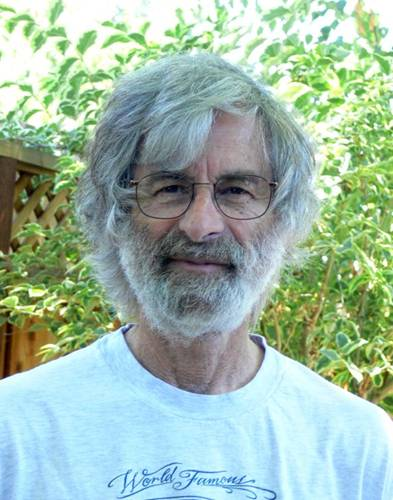
\includegraphics[
	width=\linewidth
]{lamport.jpg}

\end{minipage}}



\subsection{Tabellen}
Für die übersichtliche Darstellung von Daten sind Tabellen unerlässlich. Natürlich bietet \LaTeX\ auch dafür umfangreiche Möglichkeiten. Hier sollen aber nur die Grundlagen erklärt werden.

Erstellt werden Tabellen mit Hilfe der \texttt{tabular}-Umgebung. Dabei müssen folgende Dinge angegeben werden: Anzahl der Spalten, Ausrichtung des Zelleninhalts (linksbündig, zentriert, rechtsbündig), Rahmenlinien und natürlich der Tabelleninhalt. Abmessungen wie die Spaltenbreite werden automatisch optimal gesetzt. Eine einfache Tabelle mit zwei Spalten, zwei Zeilen und ohne Rahmenlinien sieht so aus:

\begin{minipage}{.49\linewidth}
	\lstinputlisting[caption=Tabelle]{input/tabelle.tex}
\end{minipage}
\fbox{
\begin{minipage}{.49\linewidth}
	\setlength{\parskip}{\currentparskip}
	\begin{tabular}{ll}
	Spalte 1 & Spalte 2 \\
	a & 1 \\
	b & 2
\end{tabular}
\end{minipage}}

Die gleiche Tabelle sieht mit Rahmenlinien und zentriertem Inhalt so aus:

\begin{minipage}{.49\linewidth}
	\lstinputlisting[caption=Tabelle (II)]{input/tabelle_2.tex}
\end{minipage}
\fbox{
\begin{minipage}{.49\linewidth}
	\setlength{\parskip}{\currentparskip}
	Text vor der Tabelle.

\begin{tabular}{|c|c|}
	\hline
	Spalte 1 & Spalte 2 \\
	\hline
	a & 1 \\
	\hline
	b & 2 \\
	\hline
\end{tabular}

Text nach der Tabelle.
\end{minipage}}

\begin{description}
\item[Anzahl der Spalten] Die Anzahl der Buchstaben in den eckigen Klammern direkt nach \lstinline|\begin{tabular}| (wie \texttt{\{ll\}}) definieren die Spaltenanzahl.

\item[Ausrichtung der Zellen] Dabei steht jeder Buchstabe für die Ausrichtung der Zellen innerhalb der jeweiligen Spalte: \textbf{l}eft, \textbf{c}enter, \textbf{r}ight.

\item[Rahmenlinien] Die vertikalen Striche (|, \enquote{Pipe}) fügen vertikale Rahmenlinien ein (wie in \texttt{\{|c|c|\}}). Horizontale Linien können mit \lstinline|\hline| erzeugt werden.

\item[Inhalt] Der Inhalt wird zeilenweise angegeben. Dabei markiert \& den Übergang von einer Spalte zur nächsten. Wie üblich bedeutet \verb|\\| das Ende einer Zeile.
\end{description}


\subsection{Gleitumgebungen}

Die bis jetzt gezeigten Möglichkeiten, Abbildungen und Tabellen einzufügen, sind recht unflexibel was die Positionierung innerhalb des Dokuments betrifft. Um \LaTeX\ dabei mehr Freiheit zu bieten, gibt es sogenannte \emph{Gleitumgebungen} (\texttt{figure} für Bilder, \texttt{table} für Tabellen). Der Name beschreibt sehr gut, wozu sie gedacht sind: Sie ermöglichen einem Bild oder einer Tabelle, durch das Dokument \emph{zu gleiten} und von \LaTeX\ automatisch dort positioniert zu werden, wo sie am besten hinpassen. Wenn einem also zugunsten des Gesamtlayouts nicht so wichtig ist, dass ein Bild oder eine Tabelle exakt dort erscheint, wo sie in der Quelldatei definiert wird, sollte man zu diesen Umgebungen greifen.

Außerdem bringen sie einige nützliche Features mit: der Befehl \lstinline|\caption{}| bringt an der Umgebung eine Beschreibung an, die automatisch mit dem Namen \enquote{Abbildung} oder \enquote{Tabelle} und der Nummer der Umgebung versehen wird.

\begin{minipage}{.49\linewidth}
	\lstinputlisting[caption=\texttt{figure}-Umgebung]{input/figure.tex}
\end{minipage}
\fbox{
\begin{minipage}{.49\linewidth}
	\setlength{\parskip}{\currentparskip}
	Hier ist Text vor der Gleitumgebung.

Hier ist Text nach der Gleitumgebung.

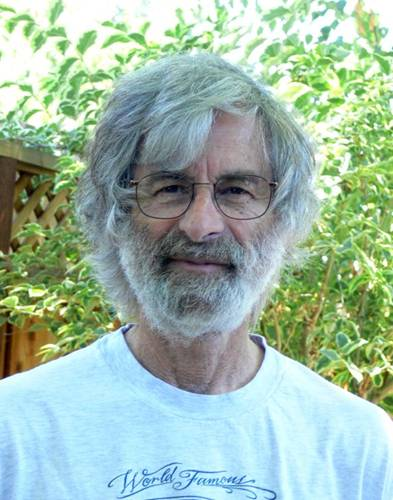
\includegraphics[
	width=\linewidth
]{lamport.jpg}
\captionof{figure}{Foto von Leslie Lamport}

\end{minipage}}

Das optionale \verb|[bth]| gibt in absteigender Priorität die Positionen an, an denen \LaTeX\ versucht, die Umgebung auf der Seite zu platzieren: \textbf{b}ottom, \textbf{t}op und \textbf{h}ere. Die Positionen werden durchprobiert, bis die ganze Seite aus typographischer Sicht \emph{schön} ist. Obwohl der untere Absatz in der Quelldatei \emph{nach} der Gleitumgebung steht, wird er im fertigen Dokument \emph{davor} angezeigt.

Mit dem Befehl \lstinline|\centering| kann der Inhalt der Umgebung zentriert werden. Ein weiteres Feature von \LaTeX\ sind die Befehle \lstinline|\label{}| und \lstinline|\ref{}|, die übrigens nicht nur im Zusammenhang mit Gleitumgebungen funktionieren:

\begin{minipage}{.49\linewidth}
	\lstinputlisting[caption=\texttt{table}-Umgebung]{input/table.tex}
\end{minipage}
\fbox{
\begin{minipage}{.49\linewidth}
	\setlength{\parskip}{\currentparskip}
	\begin{center}
\begin{tabular}{|c|c|}
	\hline
	Spalte 1 & Spalte 2 \\
	\hline
	a & 1 \\
	\hline
	b & 2 \\
	\hline
\end{tabular}
\captionof{table}{Eine Tabelle.}
\end{center}

Siehe Tabelle 1.
\end{minipage}}

\lstinline|\label{mein_label}| bringt an einem Objekt den internen Namen \enquote{mein\textunderscore label} an, auf den sich an einer beliebigen Stelle im Dokument mit \lstinline|\ref{mein_label}| bezogen werden kann. Dort wird dann automatisch die Nummer des Objekts eingefügt. Das funktioniert nicht nur mit Gleitumgebungen, sondern mit allen Objekten, die nummeriert werden, also z. B. Überschriften wie \lstinline|\section{}| und Gleichungen mit \texttt{equation}. Neben \lstinline|\ref{}| gibt es noch \lstinline|\pageref{}|, wodurch statt der Nummer die Zahl der Seite eingefügt wird, auf der das Objekt steht.

Um aus Abbildungen und Tabellen gleitende Objekte zu machen, werden sie also einfach in die entsprechende Gleitumgebung eingefügt. Anders als im ersten Beispiel verwendet gelten dabei die Positionen \verb|[htb]| als Konvention.



%-----------------------------------------------------------------------------------------------------------------------

\section{Dokumentklassen}\label{sec:klassen}
Wie am Anfang erwähnt, bestimmt die Dokumentklasse weite Teile des fertigen Layouts. Die wichtigsten Standardklassen sind \texttt{article} und \texttt{report}. Von ihnen existieren auch die moderneren Versionen \texttt{scrartcl} und \texttt{scrreprt} (\enquote{script article} und \enquote{script report}), welche einige Verbesserungen bringen. Ihre Verwendung sollte man auf jeden Fall in Betracht ziehen. Sie sind Teil der Erweiterung KOMA-Script\footnote{\url{https://www.ctan.org/pkg/koma-script}}. Die Vorlage des FSR ist ebenfalls eine Dokumentklasse, die alles speziell für Übungsserien an der MLU Benötigte zur Verfügung stellt.



%-----------------------------------------------------------------------------------------------------------------------

\pagebreak
\appendix
\section*{Anhang}
\addcontentsline{toc}{section}{Anhang}
\section{Die wichtigsten Pakete}\label{anhang:pakete}

Eine Übersicht der wichtigsten \LaTeX-Pakete und ihrer Funktion.
\begin{center}
\begin{tabular}{|l|l|l|}
\textbf{Paket} & \textbf{Funktion} & \textbf{Wichtige Optionen} \\ 
\hline 
inputenc & Interpretiere Quellcode als UTF8-kodiert & \verb|[utf8]| \\ 
fontenc & Bessere Darstellung von Umlauten etc. & \verb|[T1]| \\ 
babel & Landestypische Silbentrennung etc. & \verb|[ngerman]| \\ 
csquotes & Landestypische Anführungszeichen &  \verb|[style=german]| \\ 
lmodern & Schöne Schrift &  \\ 
amsmath, amsfonts, amssymb & Erweiterter Formelsatz &  \\
geometry & Einstellung der Seitenränder &  \\  
graphicx & Einbinden von Bildern &  \\
hyperref & Klickbare Links & \\
listings & Formatieren von Programmcode &
\end{tabular}
\end{center}



%-----------------------------------------------------------------------------------------------------------------------

\section{Wo gibt's Hilfe?}\label{sec:hilfe}
Eine Liste ausgewählter Links zu Anleitungen und Hilfen rund ums Thema \LaTeX.

\begin{description}
\item[\url{www.overleaf.com/learn}] Umfangreiche Einführung in \LaTeX\ und das Arbeiten mit Overleaf.

\item[\url{https://www3.informatik.uni-halle.de/tikiwiki/tiki-index.php}] \LaTeX-Tutorial im Info-Wiki des Instituts für Informatik der MLU (unter \enquote{Programmieren, Tools und Systeme}; Uni-intern)

\item[\url{https://tex.stackexchange.com/}] \LaTeX-Community des Stack Exchange Networks

\item[\url{https://www.informatik.uni-halle.de/studium/informatik-treff/}] Informatik-Treff des Instituts für Informatik der MLU - von Studenten für Studenten

\item[\url{https://de.wikipedia.org/wiki/Liste_mathematischer_Symbole}] Gut sortierte Liste mathematischer Symbole mit entsprechenden \LaTeX-Befehlen.

\item[\url{http://detexify.kirelabs.org/classify.html}] Diese Website erlaubt das Zeichnen eines Symbols und liefert Vorschläge für Befehle, um dieses Symbol in \LaTeX\ zu setzen.

\item[\url{www.weinelt.de/latex/}] Beschreibung aller Befehle von Standard-\LaTeX\ (nicht mehr ganz aktuell, aber immer noch sehr hilfreich und auf Deutsch).

\item[\url{www.ctan.org}] \textbf{C}omprehensive \textbf{T}eX \textbf{A}rchive \textbf{N}etwork, zentrale Anlaufstelle für Fragen zu einem bestimmten Paket.

\item[\url{https://fachschaft.mathinf.uni-halle.de/kontakt/}] Solltet ihr trotz allem mal nicht weiter kommen, könnt ihr euch natürlich auch jederzeit an uns, den FSR Mathe/Info, wenden.
\end{description}

Es gibt auch eine Vielzahl von Fachbüchern über \LaTeX, folgende zwei aus dem Bestand der Universitäts- und Landesbibliothek können wir Einsteigern besonders empfehlen:

\begin{description}
\item[H. Kopka: \LaTeX] \url{http://search.ebscohost.com/login.aspx?direct=true&db=cat06365a&AN=ulb.518786056&lang=de&site=eds-live&scope=site}

\item[M. Kohm, J.-U. Morawski: KOMA-Script] \url{http://search.ebscohost.com/login.aspx?direct=true&db=cat06365a&AN=ulb.68547044X&lang=de&site=eds-live&scope=site}
\end{description}



%-----------------------------------------------------------------------------------------------------------------------

\end{document}
